%!TEX root = ../main.tex

% Créer malware, injecter dans machine vulnérable, attendre la propagation, obtenir l'accès sur la machine sécurisé,
% une démonstration que la sécurité d'une machine dépend de la sécurité des machines avec lesquelles elle interagit.

% Tout au long de cette mémoire, nous avons parlé sur les virus, et on a cerné leurs modes de fonctionnement

Dans ce troisième chapitre, toutes les connaissances acquises durant l'étude seront mises en œuvre pour atteindre
une machine qui est supposée être sécurisée. %vérifié

La démarche que nous allons suivre est la suivante : 
\begin{itemize}
    \item Nous allons développé un Malware hybride constitué d'un virus et d'un backdoor;
    \item Le Malware sera introduit manuellement dans une machine vulnérable qui est en communication continue
        avec la machine sécurisé;
    \item Ensuit, le Malware se propagera jusqu'à la machine sécurisé sans déclencher d'alerte;
    \item Finalement, un accès total est obtenu sur la machine sécurisé par le biais du backdoor.
\end{itemize}
% nous allons développé un Malware hybride constitué d'un virus
% et d'un backdoor ; Le Malware sera introduit manuellement dans une machine vulnérable qui est en communication continue avec la machine sécurisé ; Il se propagera jusqu'à la machine sécurisé sans déclencher d'alerte ; Un 
% accès total est obtenu sur la machine sécurisé par le biais du backdoor. 

La succès de cette opération démontrera indéniablement que la sécurité d'une machine dépend toujours
de la sécurité des machines avec lesquelles elle interagit.
% machine est en communication continue avec la machine sécurisé 

% Dans cette partie de l'étude, nous allons mettre en œuvre toutes les connaissances acquises précédemment pour atteindre 
% une machine qui est supposé être sécurisé. 

% La démarche que nous allons suivre va se matérialiser dans le 
% développement d'un Malware hybride constitué d'un backdoor et d'un virus. Ce Malware sera introduit manuellement 
% dans une machine vulnérable qui est en communication continue avec la machine sécurisé. Ensuite, le Malware
% atteindra et fournira un accès sur cette dernière sans déclencher d'alerte.

% Cette démonstration a pour seul but de démontrer que la sécurité d'une machine dépend toujours de la sécurités 
% des machines avec lesquelles elle intéragit. celles avec elle
% communique

% Dans ce chapitre, nous allons mettre en œuvre toute les connaissance acquise durant cette étude pour 
% démontrer que la sécurité
% d'une machine dépend de celles avec elle communique.
\newpage

\section{Préparation de l'environnement} \label{preparation_environnement}
Dans cette section, l'environnement et les outils nécessaires pour le bon fonctionnement du projet seront installés
et préparés correctement. Il y en a en gros trois machines différentes : une machine d'attaque, une machine vulnérable,
et finalement une machine sécurisée. %vérifié

    \subsubsection{La machine d'attaque} 
    Cette machine sera équipée du système d'exploitation \emph{Kali Linux \cite{linux} Rolling} 
    (\autoref{kali_linux}), le 
    leader des systèmes de test d'intrusions. Après le téléchargement de l'image
    ISO depuis le site officiel de Kali, et l'installation de l'image sur
    une machine virtuelle, une mise à jour complète du système est faite par le biais de cette commande : 
    ``\texttt{sudo apt-get update \&\& sudo apt-get upgrade}''  %vérifié

    \begin{figure}[h!]
        \centering
        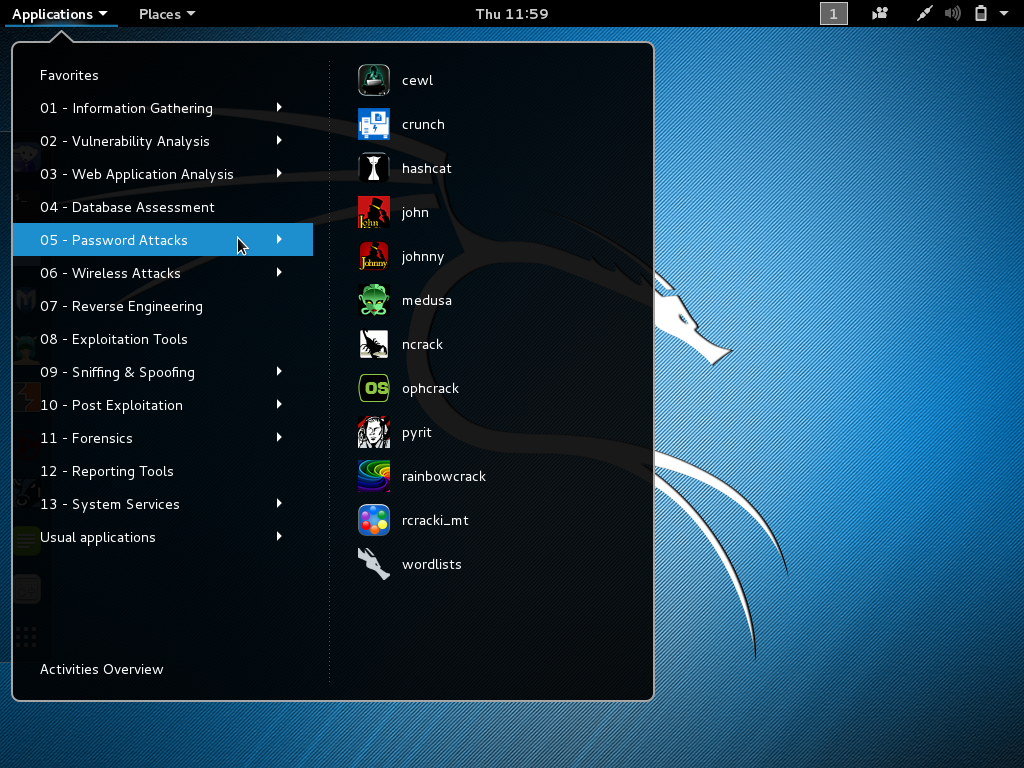
\includegraphics[width=\linewidth]{images/kali_linux.png}
        \caption{Kali Linux}
        \label{kali_linux}
    \end{figure}

    \subsubsection{La machine vulnérable} \label{machine_vulnerable} 
    Cette machine sera équipée d'une version \emph{Windows 7}  
    dotée d'un service vulnérable et d'un pare-feu désactiver. Le service vulnérable installé sur cette 
    machine est un service \emph{FTP} manipulé par le programme \emph{KONICA MINOLTA FTP Utility} 
    (\autoref{la_machine_vulnerable}). %vérifié
    \begin{figure}[h!]
        \centering
        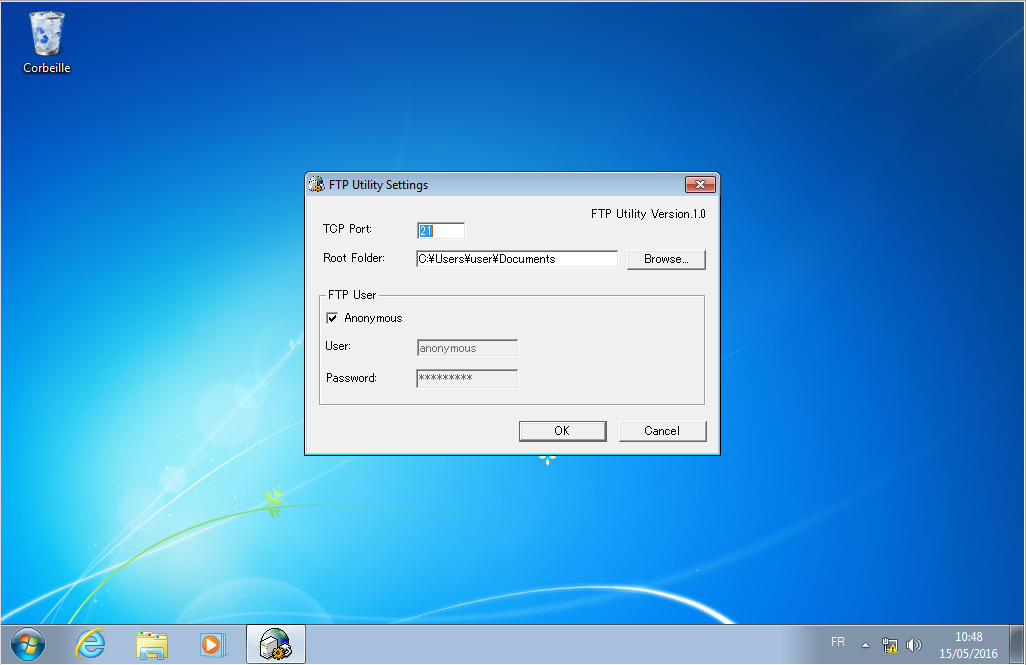
\includegraphics[scale=0.3]{images/Windows_7_2.png}
        \caption{La machine vulnérable}
        \label{la_machine_vulnerable}
    \end{figure}

    \subsubsection{La machine sécurisée} 
    Cette machine sera équipée de \emph{Windows 7} avec la dernière version de l'anti-virus \emph{Kaspersky} 
    dont la base de données a été mise à jour (\autoref{mise_a_jour_kaspersky}). %vérifié

    \begin{figure}[!h]
        \centering
        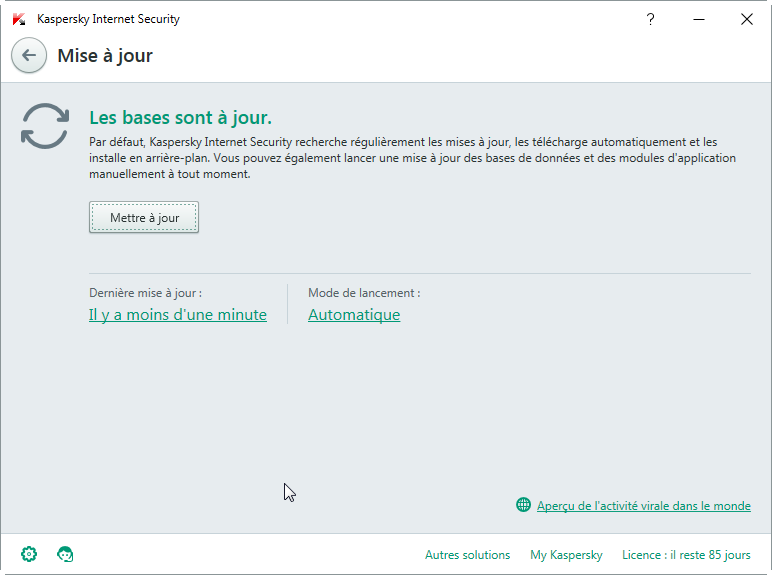
\includegraphics[width=\linewidth]{images/mise_a_jour_kaspersky.png}
        \caption{Mise à jours Kaspersky}
        \label{mise_a_jour_kaspersky}
    \end{figure}

\subsection{Réseau}
    Les trois machines seront dans le réseau \cite{reseau} dont l'adresse est \emph{172.16.178.0/24}. 
    La machine d'attaque aura l'adresse IP \emph{172.16.178.1} ; la machine vulnérable aura l'adresse IP 
    \emph{172.16.178.129} ; et finalement, la machine sécurisée aura l'adresse IP \emph{172.16.172.130}. %vérifié

    Pour voir comment le réseau a été configuré sur chaque machine, consultez \autoref{config_reseau}. %vérifié


\section{Développement}
    \subsection{Backdoor}
    Dans cette section, deux programmes seront développés : un programme qui s'exécutera sur la machine victime
    qui représentera le backdoor , et un autre qui s'exécutera sur la machine assaillante. %vérifié
    % Malgré qu'en général, exécuter un backdoor sur la machine victime et utiliser un logiciel de communication réseau
    % (comme netcat \autoref{netcat}),
    % est amplement suffisant pour obtenir un accès ; mais pour plus de compatibilité, nous allons développer 
    % les deux parties, qui sont : le backdoor et le programme qui permettra de communiquer avec.
    % le backdoor et le programme qui permettra de communiquer avec. nous allons nous même 
    % créer un programme qui permettra de communiquer avec le backdoor. 

    % Malgré que le strict minimum de cette section exige qu'on développe un backdoor (porte dérobé \autoref{backdoor})
    % qui fournira un accès à la machine victime, mais nous allons quand même développer un petit programme du côté 
    % de l'attaquant, un programme qui permettra de communiquer avec le backdoor.

    % Donc, deux programmes seront développés dans cette section : Un programme pour la machine assaillante, et 
    % un backdoor qui s'exécutera sur la machine victime.
        \subsubsection{Côté victime}
        Pour plus de discrétion, on va utiliser une technique appelée \emph{reverse connection} pour établir la connexion
        avec le backdoor. %vérifié
        % Pour éviter tous problèmes avec le pare-feu, on va utiliser une technique appelé \emph{reverse tcp}. 

        En d'autres termes, au-lieu que le backdoor ouvre un port et attend qu'on se connecte à ce port pour 
        communiquer avec lui, il va plutôt essayer d'établir une connexion vers nous. Cela permettra d'éviter la demande
        d'ouverture d'un port au pare-feu et l'éveille des soupçons de l'administrateur de la machine ; 
        par conséquence, le backdoor sera encore plus difficile à détecter.
        % Ça passe plus inaperçu, et 
        % ça évite la demande d'ouverture d'un port au pare-feu (ce qui est une activité suspecte).

        En ce qui concerne le fonctionnement du backdoor, celui-ci a été simplifié le plus possible, pour que 
        l'infection (\autoref{virus_infecteur}) passe inaperçu, et lui donner plus de chance d'échapper aux yeux des anti-virus. 
        Malgré que les fonctionnalités ont été limitées, on a donnée quand même la chance à notre backdoor 
        d'évoluer et d’intégrer plus de fonctionnalité par la suite, comment on a fait cela ? 
        L'explication est abordée ici avec la liste des fonctionnalités proposées par le backdoor : %vérifié

        \begin{description}
            \item[Accès sécurisé :] Dés le moment où le backdoor établi la connexion, un mot de passe est
                demandé par ce dernier (\autoref{backdoor_password}); si le mot de passe renseigné est correct, 
                alors l'accès est accordé, sinon la connexion est arrêter immédiatement. %vérifié

                \begin{figure}[h!]
                    \centering
                    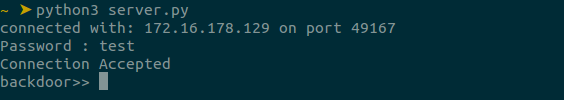
\includegraphics[width=0.9\linewidth]{images/backdoor_password.png}
                    \caption{Demande de mot de passe}
                    \label{backdoor_password}
                \end{figure}

                Pour éviter que le mot de passe soit découvert en \emph{désassemblant} l'exécutable du backdoor,
                une version hachée est conservé et utilisé pour valider le mot de passe fournie au moment de la 
                connexion. %vérifié

            \item[Accès à l'invite de commande :] Avec cette fonctionnalité, 
                chaque message envoyé par nous est redirigé vers la ligne 
                de commande de Windows, et la réponse de cette dernière est alors renvoyée.
                \begin{figure}[h!]
                    \centering
                    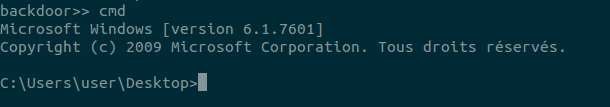
\includegraphics[width=0.9\linewidth]{images/backdoor_cmd.png}
                    \caption{Invite de commande}
                    \label{backdoor_cmd}
                \end{figure}

            \item[Envoi et réception de fichiers :] Cette fonctionnalité nous permet d'échangé des fichiers 
                avec le backdoor. Ainsi, on pourra envoyer et recevoir des fichiers depuis la machine victime.

            \item[Mettre à jours le backdoor :] Cette fonctionnalité nous permet d'étendre les fonctionnalités du
                backdoor, en le remplaçant par un autre plus sophistiqué et plus complet. Il a été précisé 
                précédemment qu'on a fait exprès de créer un backdoor simple pour éviter qu'il soit détecté ; mais 
                avec cette fonctionnalité, la seule limite de notre backdoor est notre imagination.
        \end{description}

        En ce qui concerne le lancement du backdoor, ce dernier sera lancé périodiquement par le virus, pour 
        diminuer les chances qu'une inspection des communications réseau puisse découvrir sa présence.
        % Cela permettra 
        % d'éviter la consommation inutile des ressourcesla consommation des ressources
        % Pour encore plus de discrétion, le backdoor ne sera pas en marche sans arrêt, mais il sera plutôt lancé chaque
        % période de temps par le virus.

        \subsubsection{Côté assaillant}
        Malgré qu'en général, utiliser un logiciel de communication réseau (comme netcat \autoref{netcat}) 
        est amplement suffisant pour communiquer avec 
        le backdoor. Sauf que pour exploiter toutes les fonctionnalités de ce dernier, il est indispensable 
        de développé un programme qui permettra de communiquer avec. 

        Ce programme, ou plutôt ce script python \cite{python}, écoutera sur un port donnée, et attendra la connexion du backdoor.
        Une fois cette dernière est établie, ce script permettra d'envoyer des commandes, et de recevoir leurs réponses.
        % Ce programme, ou plutôt ce script python, est extrêmement simple ; son unique tâche et d'écouter sur un port 
        % donnée, et attendre la connexion du backdoor. Une fois la connexion établie, il permettra d'envoyer 
        % des commandes, et de recevoir leurs réponses.

        \subsubsection{Backdoor amélioré}

        Ce backdoor, en plus d'intégrer toutes les fonctionnalités de l'ancien backdoor, il établie une connexion 
        crypté basé sur le protocole \emph{TLS}\footnote{Le \emph{TLS} (\emph{Transport Layer Security})
        est un protocole de sécurisation des communication réseau.}.

        Pour démonstration, le logiciel \emph{Wireshark}\footnote{\emph{Wireshark} est un analyseur de 
        paquets réseau multi-plateforme supportant plusieurs centaines de protocoles. Il permet d’examiner les 
        données qui transitent sur le réseau, et par conséquence voir le contenu des paquets en direct et en détails.} 
        a été utilisé pour montrer la différence entre la communication 
        en claire utilisé par le premier backdoor (\autoref{communication_claire})
        , et la communication cryptée utilisé par le backdoor amélioré (\autoref{communication_cryptee}).

        \begin{figure}[!h]
            \centering
            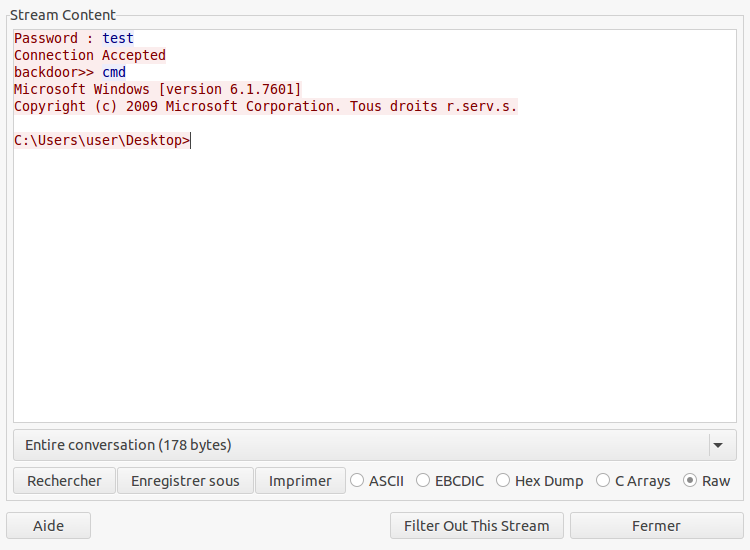
\includegraphics[width=0.8\linewidth, height=250pt]{images/communication_claire.png}
            \caption{Communication en claire}
            \label{communication_claire}
        \end{figure}
        \begin{figure}[!h]
            \centering
            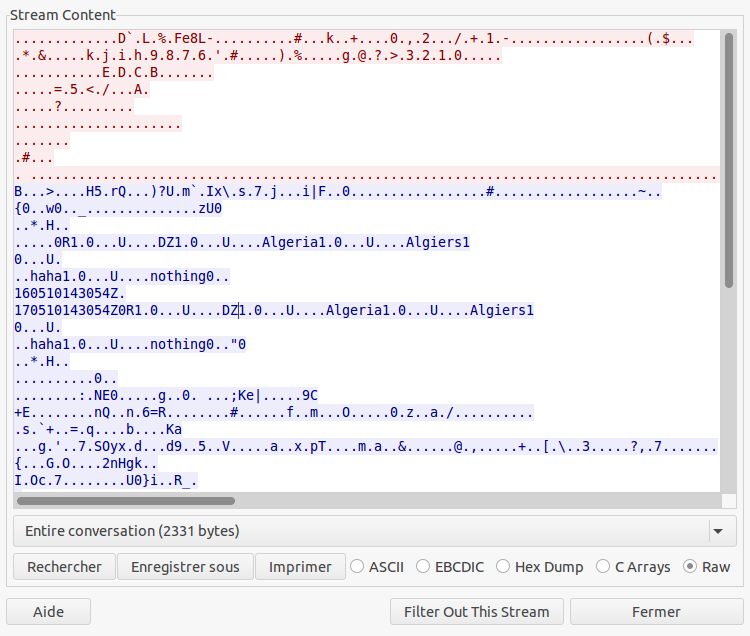
\includegraphics[width=0.8\linewidth, height=250pt]{images/communication_cryptee.png}
            \caption{Communication crypté avec le protocole TLS}
            \label{communication_cryptee}
        \end{figure}

        % non seulement il contient toutes les fonctionnalités de l'ancien backdoor, mais en
        % Ceci une petite démonstration sur la possibilité que nous offres la fonctionnalité de mise à jour. Dans cette
        % démonstration, l'ancien backdoor sera remplacé par le backdoor amélioré.
        % Le backdoor amélioré prendra la place de l'ancien backdoor dans le processus de mise à jour. 

        % En plus des fonctionnalités de l'ancien backdoor, le backdoor amélioré établira une connexion sécurisé 
        % basé sur le protocole SSL ; ainsi, l'échange sera crypté, et une inspection des paquets qui circulent sur
        % le réseau ne donnera rien de spécial.

    \subsection{Virus} \label{virus_infecteur}
    La méthode d’infection que nous allons utiliser est : l’injection de code dans un exécutable par \emph{Ajout}
    dont une définition claire a été abordée dans la \autoref{infeciton_ajout}.

    Cette technique, se base sur la manipulation de la structure PE (une définition détaillée a été donnée dans le 
    \autoref{pe_header}), nous avons donc inclus la bibliothèque \emph{Windows.h} qui contient les 
    structures et fonctions nécessaires.

    Le code se divise en deux fonctions primordiales :
    \begin{description}
        \item[WinMain :] Cette fonction est la fonction Main, dans un premier temps son rôle est de créer 
        deux espaces mémoire pour y stocker le code du Virus et du Backdoor, puis de cibler un exécutable. 
        une vérification sera faite sur sa compatibilité avec Windows 32 bits.

        Dans un deuxième temps, elle ouvre ce dernier et récupère sa structure PE. Après des calculs précis, 
        elle stocke dans une variable le Point d’Entrer Original appelé \emph{OEP} et ajoute à la fin de ce 
        fichier deux nouveaux segments; le segment qui contient le code du Virus et un autre qui contient 
        le code du Backdoor puis les crypte avec une clé prédéfinie. A la fin, elle 
        change le point d’entrer et le fait pointer vers la fonction VirusCode (\autoref{entrypoint_changement}).
        La fonction modifie aussi le \emph{loader flags}\footnote{\emph{loader flags} est un flag obsolète non
        utiliser par Windows comme expliqué dans ce lien \url{https://msdn.microsoft.com/en-us/library/windows/desktop/ms680339(v=vs.85).aspx}.} et y place notre flag d'infection. En dernier, une correction du \emph{Checksum}
        sera faite.
        
        \item[VirusCode :] Cette fonction sera le nouveau point d’enter de chaque exécutable infecté, 
            elle s’exécutera toujours en premier puis elle donnera la main au code original, 
            elle passe par trois étapes clé :

            Premièrement, puisque cette fonction n'a pas été compiler avec l’exécutable hôte, elle ne connais pas les adresse des fonctions qu'elle va utilise,
            donc une récupération de l’adresse de la bibliothèque Kernel32
            chargé avec l’exécutable hôte est primordiale et suffisant pour trouver et stocker les
            adresses des fonctions nécessaires au bon fonctionnement du code malveillant.

            Deuxièmement, elle chargera l’adresse du segment du Virus et du Backdoor, créera deux 
            emplacements mémoire et les copie dedans, puis elle les décrypte.

            Et enfin, elle créera deux fichiers exécutables dans le dossier “temp”, un contenant le Virus et 
            l’autre le Backdoor, et les exécutera. En dernier, un appel vers le point d’entrer original sera fait
            pour redonner la main à l'exécutable hôte, ce qui permettra d'éviter l'éveille des soupçons.

    \end{description}

\newpage

    \begin{figure}[H]
        \centering
        \begin{subfigure}{0.9\textwidth}
            \centering
            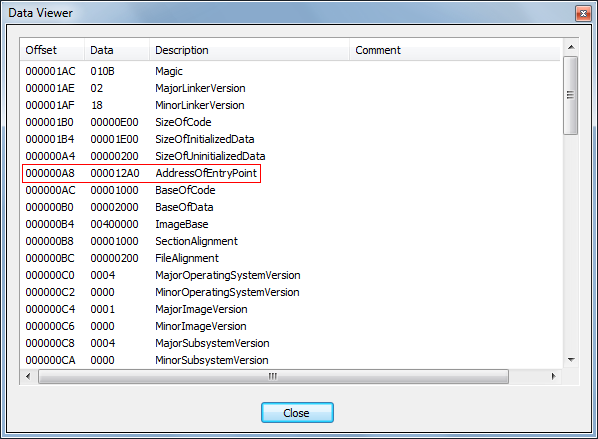
\includegraphics[width=\textwidth]{images/entrypoint_avant.png}
            \caption{Point d'entrée avant infection}
            \label{entrypoint_avant}
        \end{subfigure}
        \hfill
        \begin{subfigure}{0.9\textwidth}
            \centering
            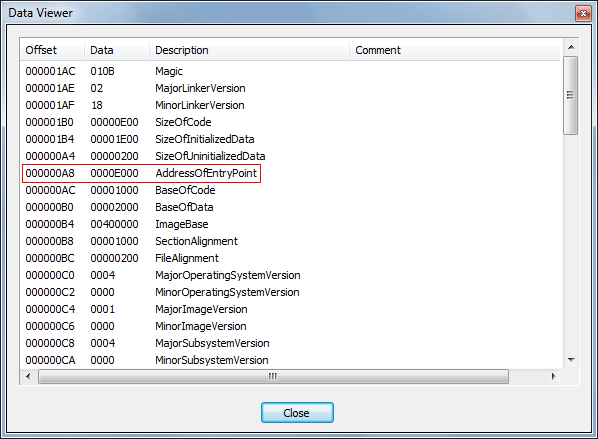
\includegraphics[width=\textwidth]{images/entrypoint_after.png}
            \caption{Point d'entrée après infection}
            \label{entrypoint_apres}
        \end{subfigure}
        \hfill
        \caption{Changement du point d'entrée de l'exécutable}
        \label{entrypoint_changement}
    \end{figure}

    Nous citerons aussi que ce Virus infecte les fichiers exécutables des clés USB connecté à la machine.
    La particularité majeure de notre Virus est qu’il utilise des API native, et qu’il ne peut pas être 
    déboguer, une démonstration est montrer dans la figure suivante:

\section{Exploitation} \label{exploitation}
Cette section sera consacré à l'exploitation de la machine vulnérable, et l'obtention d'un accès à distance
sur cette dernière. On commencera par une bref présentation des outils utilisés pour une meilleur compréhension
de cette section.
    \subsection{Présentation des outils}
    \begin{description}
        \item[netcat :] \label{netcat}
            C'est un outil utilisé en ligne de commande, et qui permet l'ouverture des connexions
            réseau, que ce soit \emph{TCP} \cite{reseau} ou \emph{UDP} \cite{reseau}. En raison de sa polyvalence,
            il est aussi appelé le \emph{couteau suisse} du réseau.

            Pour se connecter à un serveur sur un port donnée, il faut donner à \emph{netcat} deux paramètres qui sont 
            l'adresse du serveur et le port qu'utilise le serveur. Exemple :
            \begin{lstlisting}[language=bash] 
            $ netcat www.google.com 80
            \end{lstlisting}

            Dans le côté serveur, pour mettre netcat en écoute sur un port, il faut préciser deux options qui sont 
            `\emph{-l}' pour dire à netcat d'écouter, et `\emph{-p \ul{port}}' pour préciser le port d'écoute.
            Exemple :
            \begin{lstlisting}
            # netcat -l -p 80   
            \end{lstlisting}

        \item[Metasploit :] C'est un \emph{Framework} de testes de pénétrations \emph{open source} utilisé pour 
            tester la robustesse des machines en matière de sécurité. Il est composé essentiellement de charges 
            et d'exploits. 

        \item[msfvenom :] \label{msfvenom} C'est un générateur et encodeurs de charges. Il est utile pour une utilisation plus manuelle
            des charges, car il permet de générer ces dernières dans plusieurs format (des exécutables, pour un 
            script python \ldots{}). 

            Plusieurs paramètres sont à utiliser pour obtenir des charges plus performantes. Parmi ces options on y
            trouve :
            \begin{description}
                \item[-a \ul{architecture} :] L'architecture du système dont la charge est destiné
                    (x86 ou x64).
                \item[--plateform \ul{plateforme} :] Le système attaqué (Windows, Mac, Linux, Android
                \ldots{}).
                \item[-p \ul{charge} \ul{options\_de\_la\_charge}:] La charge et les options utilisés 
                    pour générer celle-ci.
                \item[-e \ul{encodage} :] L'encodage utilisé pour générer la charge.
                \item[-b \ul{mauvais\_octets} :] Les octets à éviter pendant la génération de la charge.
                \item[-f \ul{format} :] Format de la charge (exécutable, python, perl \ldots{}).
            \end{description}

        \item[meterpreter :] \label{meterpreter}C'est une charge avancée et extensible développé par les développeurs de 
            \emph{Metasploit}. Elle est utilisé par ce dernier pour donner un accès plus étendu et plus 
            complet à une machine exploitable. 
    \end{description}

    \subsection{La vulnérabilité}
    Le programme vulnérable qu'on va exploiter se nomme \emph{Konica Minolta FTP Utility} (\autoref{konica_minolta}). 
    C'est un programme qui utilise le protocole \emph{FTP}\footnote{Le \emph{FTP} est un protocole destiné
    à l'échange informatique des fichiers sur un réseau.} pour la réception des données depuis des appareils 
    compatibles. La version vulnérable, qui est la \emph{version1.0} 
    (la dernière jusqu'à maintenant), peut être obtenu depuis ce lien 
    \url{https://www.exploit-db.com/apps/6388a2ae7dd2965225b3c8fad62f2b3b-ftpu_10.zip}.
    % La version vulnérable du programme est la \emph{version 1.0} (qui est la dernière version 
    % jusqu'à maintenant), cette version peut être obtenu depuis ce lien 
    % \url{https://www.exploit-db.com/apps/6388a2ae7dd2965225b3c8fad62f2b3b-ftpu_10.zip}.
    % pour recevoir des données 
    % Le service vulnérable qui a été installé est un service \emph{ftp} manipulé par le programme 
    % \emph{Konica Minolta FTP Utility}. 

    \begin{figure}[h]
        \centering
        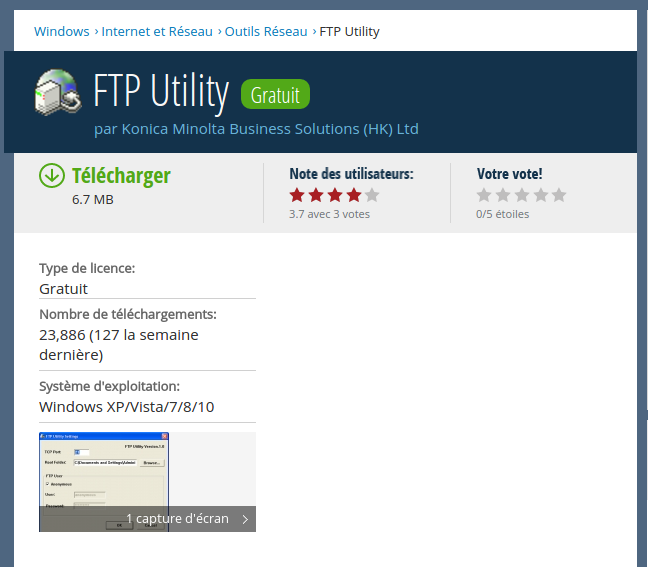
\includegraphics[width=0.8\linewidth]{images/konica_minolta.png}
        \caption{Konica Minolta FTP Utility}
        \label{konica_minolta}
    \end{figure}

    La vulnérabilité découverte dans ce programme est un débordement de tampon (\autoref{buffer_overflow}), 
    elle a été publié le 21 Janvier 2016 sur le site d'\emph{Exploit Database} 
    \footnote{\emph{Exploit Database} est un site qui se charge d'archiver les exploits publics et les 
    logiciels vulnérables correspondants. Ce site dont le lien est \url{www.exploit-db.com} est développé 
    par les testeurs d'intrusions et les chercheurs de vulnérabilités.} par un contributeur surnommé \emph{TOMIWA}.
    % La vulnérabilité découverte, qui est un débordement de tampon (\autoref{buffer_overflow}), a été publié le 11
    % Janvier 2016 sur le site d'\emph{Exploit Database}\footnote{\emph{Exploit Database} est un site qui se charge
    % d'archiver les exploits publics et les logiciels vulnérables correspondants. Ce site dont le lien est 
    % \url{www.exploit-db.com} est développé par les testeurs d'intrusions et les chercheurs de vulnérabilités.} 
    % par une personne surnommé \emph{TOMIWA}.

    % La vulnérabilité est présente dans la \emph{version 1.0} (qui est la dernière version jusqu'à maintenant) du
    % programme. Cette version peut être obtenu depuis ce lien 
    % \url{https://www.exploit-db.com/apps/6388a2ae7dd2965225b3c8fad62f2b3b-ftpu_10.zip}.

    \subsection{L'exploit}
    Le script qui permet d'exploiter cette vulnérabilité peut être récupérer depuis ce lien 
    \url{https://www.exploit-db.com/exploits/39215/}.
    Ce script \emph{python} \cite{python} se divise en deux parties :
    \begin{description}
        \item[Exploit :] Cette partie du script permet en quelque sorte de préparer le programme vulnérable à 
            recevoir le code malveillant pour l'exécution. Cette partie n'est pas à modifier, car elle a été développé
            après une étude approfondie du programme vulnérable.

        \item[Charge :] Cette partie du script représente le code qui sera exécuté sur l'application vulnérable. 
            Cette partie peut être remplacé par la charge désiré par l'attaquant.
            % L'exploit téléchargé depuis ce lien \url{https://www.exploit-db.com/exploits/39215/} vient avec une charge
            % par défaut, qui est un \emph{reverse shell}.% Pour notre démonstration, on ne va pas utiliser 
            % la charge par défaut, mais on va plutôt utiliser une autre charge qui permet d'exécuter un programme 
            % beaucoup plus puissant, qui est \emph{meterpreter}. 
    \end{description}

    Le script va se connecter à la machine victime sur le port 21 (\autoref{execution_script_exploitation}). 
    La charge qu'utilise le 
    script va ordonné à la machine qu'elle donne un reverse shell en se reconnectant à la machine de l'attaquant 
    sur le port 4444. Pour intercepter ce reverse shell, et pouvoir communiquer avec
    la machine victime, il faut ordonner à netcat d'écouter sur le port 4444 (\autoref{obtention_reverse_shell}).

    \begin{figure}[h!]
        \centering
        \begin{subfigure}{0.9\textwidth}
            \centering
            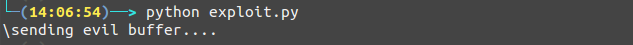
\includegraphics[width=\textwidth]{images/exploit_python.png}
            \caption{Exécution du script d'exploitation}
            \label{execution_script_exploitation}
        \end{subfigure}
        \hfill
        \begin{subfigure}{0.9\textwidth}
            \centering
            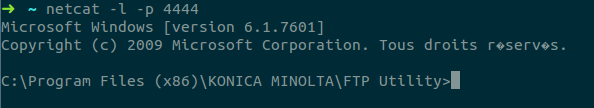
\includegraphics[width=\textwidth]{images/reverse_shell.png}
            \caption{Obtention du reverse shell}
            \label{obtention_reverse_shell}
        \end{subfigure}
        \hfill
        \caption{Exploitation avec la charge d'origine}
        \label{exploitation_avec_charge_origine}
    \end{figure}

    La charge par défaut de ce script est une charge un petit peu limitée, donc nous allons nous en servir 
    de \emph{msfvenom} pour générer la charge \emph{meterpreter} (\autoref{generation_charge}) et l'utiliser 
    dans le script d'exploitation.
    \begin{figure}[h]
        \centering
        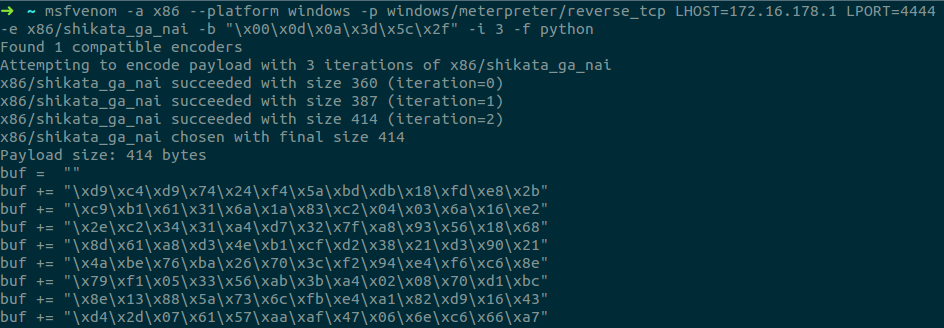
\includegraphics[width=\linewidth]{images/msfvenom.png}
        \caption{Génération de la charge}
        \label{generation_charge}
    \end{figure}

    \subsection{Obtention d'accès}
    Pour la charge utilisé précédemment, il a suffit d'utiliser netcat pour intercepter la connexion et communiquer
    avec la machine victime. Mais meterpreter exige des techniques plus poussées pour pouvoir faire cela, 
    donc nous allons faire appel aux services de Metasploit pour accomplir cette tâche.
    On commence par lancer Metasploit en mode console (\autoref{msfconsole}) par le biais de la commande 
    `\emph{msfconsole}'. Après, on effectue les manipulations nécessaires (\autoref{config_metasploit})
    pour pouvoir intercepter les réponses de meterpreter.

    \begin{figure}[H]
        \centering
        \begin{subfigure}{0.9\textwidth}
            \centering
            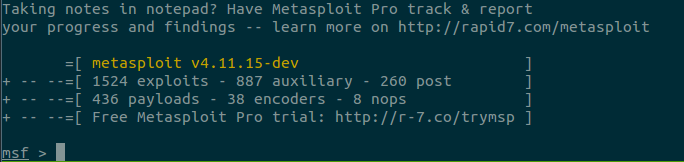
\includegraphics[width=\textwidth]{images/msfconsole.png}
            \caption{Lancement de Metasploit}
            \label{msfconsole}
        \end{subfigure}
        \hfill
        \begin{subfigure}{0.9\textwidth}
            \centering
            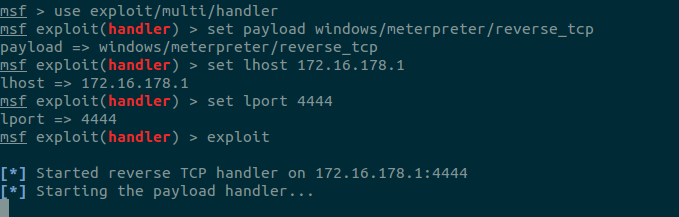
\includegraphics[width=\textwidth]{images/ecoute_msf.png}
            \caption{Configuration de Metasploit}
            \label{config_metasploit}
        \end{subfigure}
        \hfill
        \caption{Préparation de Metasploit}
        \label{prepration_metasploit}
    \end{figure}

    Maintenant, il ne reste plus qu'à lancer le script d'exploitation qu'on a modifié et obtenir un accès à la 
    machine exploité (\autoref{obtention_accees_meterpreter}).

    \begin{figure}[H]
        \centering
        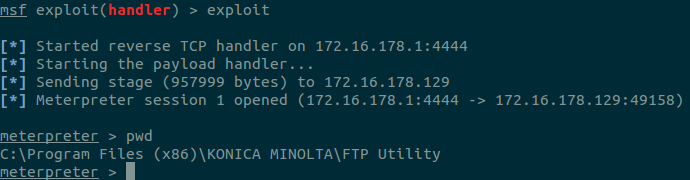
\includegraphics[width=\linewidth]{images/meterpreter.png}
        \caption{Obtention de l'accès avec meterpreter}
        \label{obtention_accees_meterpreter}
    \end{figure}

\section{Teste de propagation}
Cette partie contiendra une simulation de propagation du Malware développée au cours de ce projet, et 
l'infection des machines d'une entreprise virtuel,

Pour cela, nous procédons au test sur l’environnement cité auparavant dans la \autoref{preparation_environnement}.

Tout d'abord, nous exploitons la vulnérabilité présente dans la machine de faible sécurité, pour avoir accès au Shell de cette dernière (comme expliqué dans la \autoref{exploitation}), de ce fait, nous envoyons notre Malware puis nous l’exécutons (\autoref{launch_virus})

\begin{figure}[H]
    \centering
    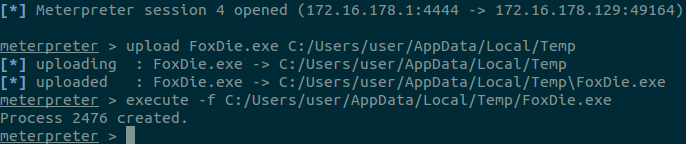
\includegraphics[width=\linewidth]{images/exec_virus.png}
    \caption{Envoi et exécution du virus}
    \label{launch_virus}
\end{figure}
Cela infectera la machine et tout fichier exécutable contenu dans des périphériques de stockage externe qui sont, ou qui vont  être connectes à cette machine.  Nous pouvons constater que le processus de notre Virus est en execution sur la machine, et nous pouvons aussi observer qu'à chaque minute, le backdoor est exécuté (\autoref{process_backdoor}).

\begin{figure}[H]
    \centering
    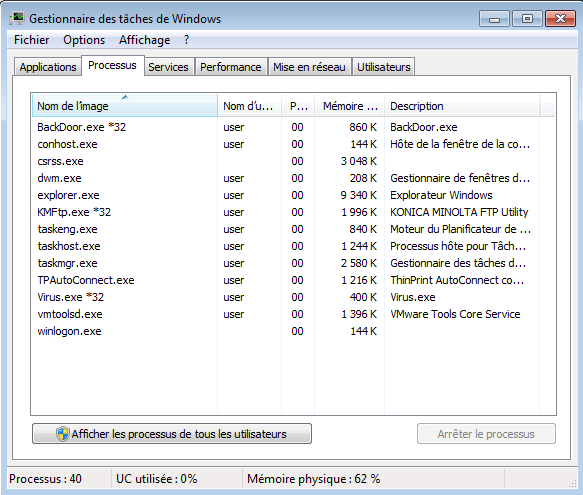
\includegraphics[width=\linewidth]{images/processus_backdoor.png}
    \caption{Processus du backdoor}
    \label{process_backdoor}
\end{figure}

Pour la deuxieme étape de notre test, nous connectons une clé usb contenant plusieurs fichiers, dont des exectuables et autres (\autoref{avant_infection}). A ce titre nous pouvons constater que la taille des executables s'agrandit de 144 Ko (\autoref{apres_infection}), cela veux dire que les deux segments (le virus et le backdoor) ont été ajouté correctement .

\begin{figure}[H]
    \centering
    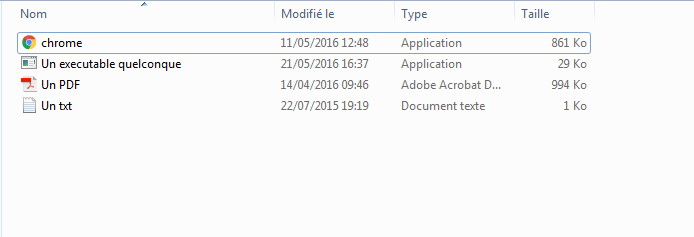
\includegraphics[width=\linewidth]{images/avant_infeciton.png}
    \caption{Avant Infection}
    \label{avant_infection}
\end{figure}

\begin{figure}[H]
    \centering
    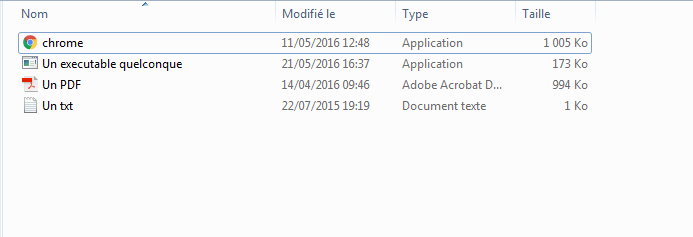
\includegraphics[width=\linewidth]{images/apres_infection.png}
    \caption{Après Infection}
    \label{apres_infection}
\end{figure}

Nous prenons cette clé, puis nous la connectons à la machine qui est hautement sécurisée. Nous essayons de l'analyser avec le fameux Anti Virus \emph{Kaspersky} qui après analyse indique que tous les fichiers contenus dans la clé sont sains et non infectés (\autoref{scan_cle}). Nous procédons alors à l’exécution de l'un des fichiers exécutable comme le ferait n'importe quel usager utilisant un Anti Virus.

\begin{figure}[H]
    \centering
    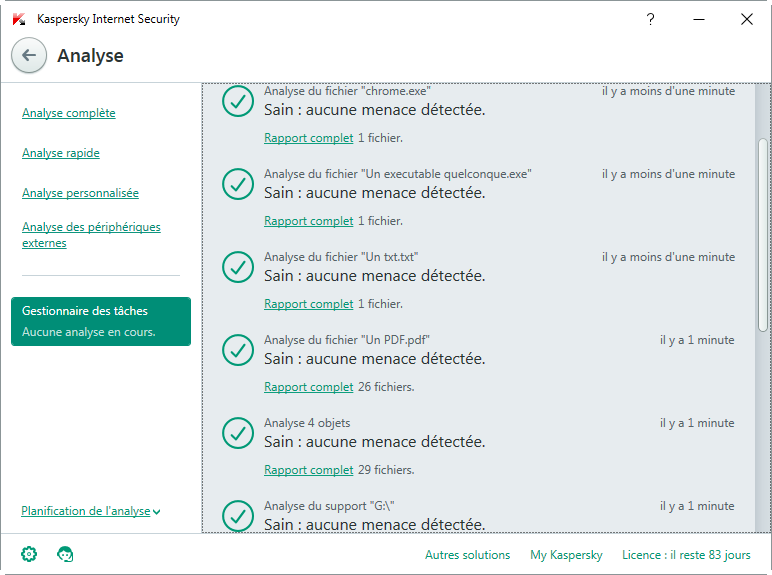
\includegraphics[width=\linewidth]{images/scan_by_antivirus.png}
    \caption{Scan de la clé USB}
    \label{scan_cle}
\end{figure}

A cet effet, le code malveillant contenu dans le logiciel infecté s’exécute en premier comme cité dans la 
\autoref{virus_infecteur}, et fera la tâche qui lui a été assignée.

Par la suite, nous lançons  notre serveur dans notre machine en écoute comme le montre la figure suivante, et on attend que le backdoor qui s’exécute dans la machine sécurisée se connecte vers ce dernier. Après un laps de temps, la connexion s'effectue (\autoref{connect_backdoor}), ce qui nous donne finalement un accès total à la machine réputée comme étant protégée et inviolable.

\begin{figure}[H]
    \centering
    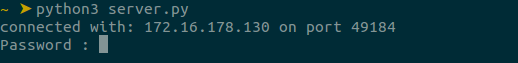
\includegraphics[width=\linewidth]{images/backdoor_connect.png}
    \caption{Connexion du backdoor à notre serveur}
    \label{connect_backdoor}
\end{figure}

\section{Conclusion}
A la fin de chapitre final, nous avons réuissi à dévellopé un Malware hybride. Ce Malware a prouvé son efficacité
contre les anti-virus, et il a réussi à atteindre la machine sécurisé par le biais d'une propagation furtive.

A la fin de chapitre, une machine sécurisé à été atteinte par notre Malware. Pour 
parvenir à cet objectif, nous avons commencé par développé le Malware hybride, puis, il a été 
injecté dans la machine vulnérable par le biais de l'exploitation d'une faiblesse dans cette dernière. 
Enfin, le Malware a réuissi à propager jusqu'à la machine sécurisé en car elle est en communication 
continue avec la machine qu'on a exploité précédemment.

% A la fin de chapitre final, nous avons réussi à atteindre une machine sécurisé par le moyen d'un Malware que nous 
% avons développé. Ce Malware s'est propagé jusqu'à atteindre 

% A la fin de ce chapitre final nous avons développé le Malware avec succès, tester son efficacité contre les Anti-Virus, et tester sa propagation vers des machines plus sécurisé.
% Il reste qu’il est toujours possible d’optimiser l’efficience du Malware au vue de sa capacité a évité les Anti-Virus.
